\begin{figure}
  \centering
  \includegraphics[width=.95\linewidth]{figures/aws-variation.pdf}
  \caption{Bandwidth measurement between Amazon EC2 sites (from Ireland to
    California). Note the time-series plot has a resolution of 30 minutes.}
  \label{fig:bw}
\end{figure}

\section{Motivation}
\label{sec:motivation}

In this section, we examine the gap between high application demands and limited
wide-area bandwidth. We then show that neither application-specific
optimizations nor manual policies solve the problem.

\subsection{Wide-area Streaming Applications}
\label{sec:wide-area-streaming}

\paraf{Video Surveillance:} We envisage a city-wide monitoring system that
aggregates camera feeds (both stationary ground cameras and moving aerial
vehicles) and analyzes video streams in real-time for surveillance, anomaly
detection or business intelligence~\cite{oh2011large}. Traditionally, humans are
involved in analyzing abnormal activities. Recent advances in computer vision
and deep learning has dramatically increased the accuracy for visual scenes
analysis, such as pedestrian detection~\cite{dollar2012pedestrian}, vehicle
tracking~\cite{coifman1998real}, or facial recognition to locate people of
interest~\cite{parkhi2015deep, Lu:2015:SHF:2888116.2888245}.

\para{High-frequency IoT Sensors:} Traditionally, environmental sensors are slow
and not data-intensive~\cite{atzori2010internet}. Increasingly, high-frequency,
high-precision sensors are being deployed. For example, the uPMUs monitor the
electrical grid with a network of 1000 devices; each produces 12 streams of 120
Hz high-precision values accurate to 100 ns. This amounts to 1.4 million points
per second that requires specialized timeseries
database~\cite{andersen2016btrdb}.

\para{Industrial Monitoring:} Large organizations today are managing 10--100s of
datacenters (DCs) and edge clusters worldwide~\cite{calder2013mapping}. While
most log analysis today runs in a batch mode and on a daily basis, there is
trend in analyzing logs in real-time for quicker optimization. For example, a
content distribution network (CDN) can improve the overall efficiency by
optimizing data placement if the access logs can be processed in real-time.

% We consider the practical issues with deploying these applications in the
% wide-area. Our stand is that these applications face a bigger network challenge.
% Data generated from the edge often fail to be delivered to the the processing
% site because of the scarce and variable bandwidth capacity in the
% wide-area. Once they arrive, existing stream processing systems can easily
% manage a large cluster and perform data analytics at real-time.

\begin{figure*}
  \centering
  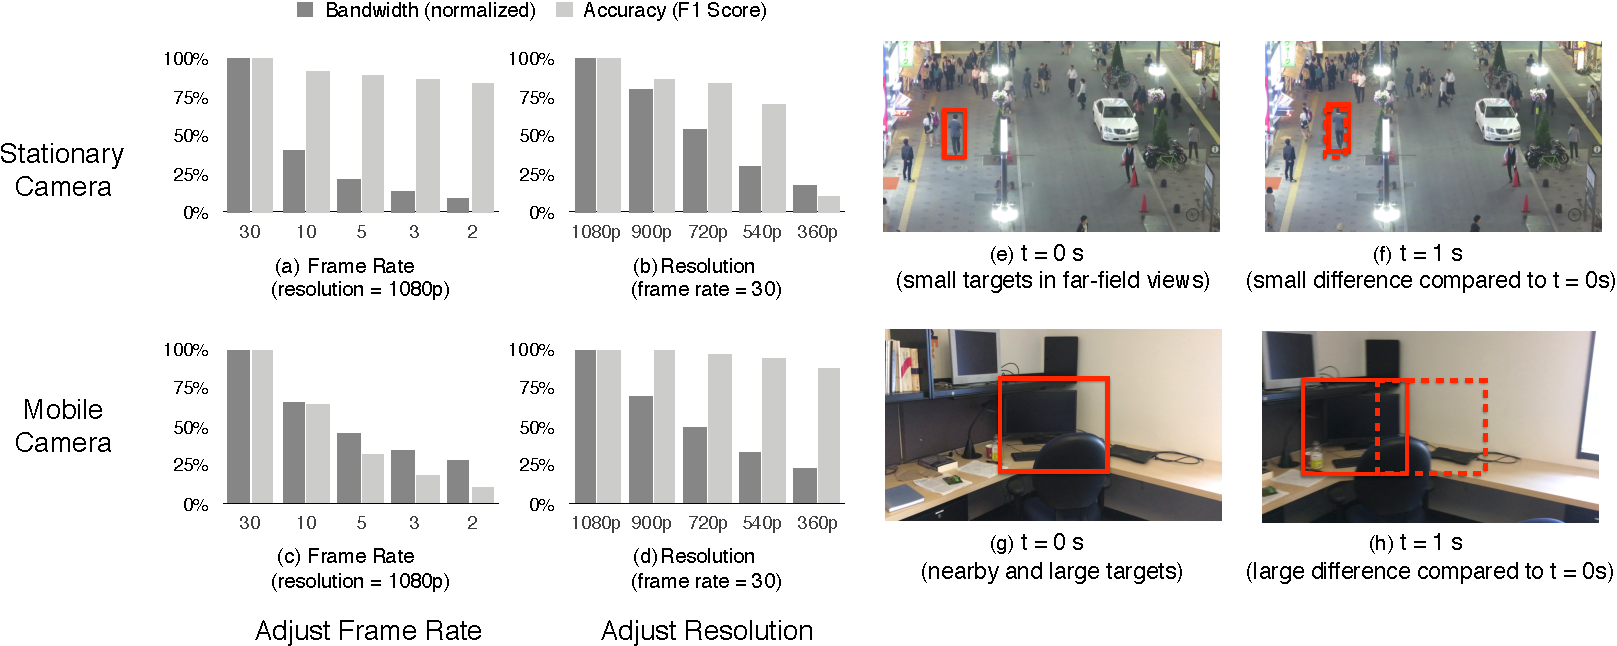
\includegraphics[width=1.0\linewidth]{figures/motiv-app-specific.pdf}
  \caption{Application specific adaptations doesn't generalize. There are often
    multiple dimensions to explore. Degradation has different impact along
    different dimension}
  \label{fig:app-specific}
\end{figure*}

\subsection{Wide-area Bandwidth Characteristics}
\label{sec:wide-area-bandwidth}

Recent work on WAN-aware systems have all demonstrated the insufficiency and
cost nature of wide area bandwidth~\cite{pu2015low, vulimiri2015global}. Figure
2 in Gaia~\cite{hsieh17gaia} shows that the WAN bandwidth is 15x smaller than
the LAN bandwidth on average, and up to 60x smaller in the worst case.

In addition to the scarcity, WAN bandwidth also has great variability. We
conducted a day-long measurements using iPerf~\cite{iperf3} to measure the
pair-wise bandwidth between four Amazon EC2 sites. We observed large variance in
the measured bandwidth and one such pair of sites is shown
in~\autoref{fig:bw}. There exist occasions when the available bandwidth is
almost halved.

The back-haul links between EC2 sites are better (if not at least
representative) in comparison to the general wide-area links. Similar variations
have also been reported in wireless network~\cite{biswas2015large}, ISP
network~\cite{grover2013peeking} and cellular
network~\cite{nikravesh2014mobile}. The scarce and varying nature poses real
challenge to the realization and successful deployment of wide-area streaming
applications.

\subsection{Making the Case for a System Approach}
\label{sec:making-case-sys-approach}

This motivates us to take a system-level approach that synthesize different
adaptation strategies for different queries and contexts.

\para{Application-specific solutions don't generalize.} One class of the
wide-area streaming analytics are processing videos to analyze visual
scenes. While adaptive streaming exist in certain application domain, there has
not been a general solution. Consider video streaming applications that have
been extensively studied in the literature. There are a plethora of encoding
techniques~\cite{richardson2011h, grange2016vp9} with adaptive
strategies~\cite{yin2015control, michalos2012dynamic, pantos2016http}, however,
their primary goal is to optimize end-user quality of experience (QoE)

Video streaming analytics often have different goals, therefore entail different
adaptive strategies. For example, many computer vision detection algorithms rely
on the edge information~\cite{canny1986computational, lowe2004distinctive,
  viola2001rapid} while object tracking applications works best when the
inter-frame difference is small~\cite{allen2004object}.

Similar applications with a different context requires different strategies. We
illustrate this point with an example in \autoref{fig:app-specific}. In object
detection deployed with a ground stationary camera. When taking pedestrian
walking speed into consideration, a high frame rate is not necessary. But
because these surveillance cameras are far from the target, it's crucial to have
a high-resolution and sharp image. On the other hand, when deployed with a
mobile phone, due to the movement of the camera, reducing frame rate will
introduce significant errors.

\para{Manual polices are sub-optimal.} We consider manual policies for
adaptation. JetStream~\cite{rabkin2014aggregation} offers an example:
\textit{``if bandwidth is insufficient, switch to sending images at 75\%
  fidelity, then 50\% if there still isn't enough bandwidth. Beyond that point,
  reduce the frame rate, but keep the images at 50\% fidelity.''} This approach
has the following issues.

Precision. These policies are developer heuristics and not backed up by
measurements. There is no direct association of the application accuracy with
the 75\% fidelity configuration. Besides, it's unclear about how much the policy
would affect the data size. For example, reducing the frame rate by 50\%
\textit{seems} to half the data rate. But when the video is encoded with H.264,
frame rate's reduction leads to bigger inter-frame differences, resulting in a
larger P-frame size.

%% \autoref{fig:h264} illustrates this complex relationship with an example of
%% H.264 encoding under four different frame rates.

It's not scalable. The strawman solution quickly leads to too many policies when
multiple degradation operations are involved or a fine-grained control is
desired. This manual process becomes tedious and error-prone. When too few rules
are provided, the application may oscillate between aggressive rules and
conservative rules.

The abstraction is too low-level. Developers are forced to manually study and
measure the impact of individual degradation policy, prohibiting its wide
adoption in practice.

%%% Local Variables:
%%% mode: latex
%%% TeX-master: "sosp17"
%%% End:
